% % Preamble BEGINN %%%%%%%%%%%%%%%%%%%%%%%%%%%%%%%%%%%%%%%%%%%%%%%%%%%%%%%%%

%%% Preamble (Dokumentenklasse)
% ------------------------------------------------------------------------
% LaTeX - Preambel ******************************************************
% ------------------------------------------------------------------------
% Dokumentklasse (Koma Script)
% ------------------------------------------------------------------------
% basiernd auf www.matthiaspospiech.de/latex/vorlagen Diplomarbeit kompakt
% ========================================================================
\documentclass[%
   %draft,            % Entwurfsstadium
   final,             % fertiges Dokument
   12pt,              % Schriftgroesse der Grundschrift
   bigheadings,       % gro�e �berschriften
   ngerman,           % wird an andere Pakete weitergereicht
   a4paper,           % Papierformat
   BCOR5mm,          % Bindekorrektur: Zus�tzlicher Rand auf der Innenseite
   DIV14,            % Seitengr��e (siehe Koma Skript Dokumentation !)
   1.1headlines,     % Zeilenanzahl der Kopfzeilen
   pagesize,         % Schreibt die Papiergroesse in die Datei.
   oneside,          % Einseitiges Layout
%   twoside,          % Zweiseitiges Layout
   openright,        % Kapitel beginnen immer auf der rechten Seite
   titlepage,        % Titel als einzelne Seite ('titlepage' Umgebung)  
   headsepline,      % Linie unter Kolumnentitel ()
%   plainheadsepline, % Linie unter Kolumnentitel () plain Seitenstil
   nochapterprefix,  % keine Ausgabe von 'Kapitel:'
   bibtotoc,         % Bibliographie ins TOC
%	bibtotocnumbered, % Bibliographie ins TOC mit Kapitelnummer
   tocindent,        % eingereuckte Gliederung
   listsindent,      % eingereuckte LOT, LOF
   pointlessnumbers, % �berschriftnummerierung ohne Punkt, siehe DUDEN !
   cleardoubleempty, % Leere linke Seite bei Zweiseitenlayout vor Kapitel
   fleqn,            % Formeln werden linksbuendig angezeigt
%   parindent,        % Absatz mit Einzug (Standard)
   halfparskip,      % Absatz halbe Zeile Abstand
%   parskip,          % Absatz ganze Zeile Abstand
]{scrbook}%     Klassen: scrartcl, scrreprt, scrbook


%%% Alle Namen usw. im Titel und im hyperref-Paket
% ------------------------------------------------------------------------
% LaTeX - Preambel ******************************************************
% ------------------------------------------------------------------------
% pre-work
% ========================================================================
% % ToDo kennzeichnen
\newcommand{\workTodo}[1]{\textcolor{red}{todo: #1}}

% % F�r Datum und Zeit in Fusszeile
% % !!!Inhalt bei Fertigstellung der Arbeit l�schen
\newcommand{\workMarkDateTime}{}

% % Alle Namen werden im Titel und im hyperref-Paket eingetragen
% % !!! Ueberall f�r <Wert> das Entsprechende eintragen

 % <Typ> Studienarbeit, Dipolmarbeit, Studienarbeit oder Bachlor-Abschlussarbeit
\newcommand{\workTyp}{\workTodo{<Typ>}\xspace}

 % <Titel> der Arbeit
\newcommand{\workTitel}{Tracing-Tool zur Analyse von IO auf HPC-Systemen\xspace}

 % <Studiengang> z.B. Kommunikationstechnik
\newcommand{\workStudiengang}{\workTodo{<Studiengang>}\xspace}

% <Semester> mit Jahr z.B. Sommersemester 2008  
\newcommand{\workSemester}{\workTodo{<Semester>}\xspace}

% <Name> des Studenten
\newcommand{\workNameStudent}{\workTodo{<Name>}\xspace}

% <Pruefer> Name des pr�fenden (betreuenden) Professor an der Hochschule
\newcommand{\workPruefer}{Prof. Dr.-Ing. Rainer Keller\xspace} 


% %%% Nur bei Abschluss-Arbeiten

% <Datum> der Abgabe der Arbeit (Eidesstatliche Erkl�rung)
\newcommand{\workDatum}{\today\xspace}

% <Zweitpr�fer>
\newcommand{\workZweitPruefer}{\workTodo{<Zweitpr�fer>}\xspace}

% <Zeitraum>
\newcommand{\workZeitraum}{\workTodo{<Zeitraum>}\xspace}


% %%% Nur bei Industrie-Arbeiten:

% <Firma>
\newcommand{\workFirma}{\workTodo{<Firma>}\xspace}

% <Betreuer in der Firma>
\newcommand{\workBetreuer}{\workTodo{<Betreuer in der Firma>}\xspace}

% Firmenlogo Name hier anpassen, Gr��e (wenn m�glich) nicht �ndern
\newcommand{\workFirmenLogo}{
\includegraphics[width=3cm]{fig/aa-titel/bwhpc}} 


%%% Preamble (Pakete)
% ------------------------------------------------------------------------
% LaTeX - Preambel ******************************************************
% ------------------------------------------------------------------------
% Packages
% ------------------------------------------------------------------------
% basiernd auf www.matthiaspospiech.de/latex/vorlagen Diplomarbeit kompakt
% ========================================================================

% Inhalt:
% 1. Einige Pakete muessen unbedingt vor allen anderen geladen werden
% 2. Fonts Fonts Fonts
% 3. Math Packages
% 4. Symbole
% 5. text related packages
% 6. Pakete zum Zitieren
% 7. PDF related packages
% 8. Tables (Tabular)
% 9. figures and placement
% 10. verbatim packages
% 11. science packages
% 12. layout packages
% 13. tikz packages
% 14. Tables (longtabu)

% ~~~~~~~~~~~~~~~~~~~~~~~~~~~~~~~~~~~~~~~~~~~~~~~~~~~~~~~~~~~~~~~~~~~~~~~~
% Encoding der Dateien (sonst funktionieren Umlaute nicht)
% Empfohlen latin1, da einige Pakete mit utf8 Zeichen nicht
% funktionieren, z.B: listings, soul.

\usepackage[latin1]{inputenx} % ISO-8859-1
%\usepackage[ansinew]{inputenx} % Windows-Standard (CP1252) (baut auf ISO 8859-1 und ISO 8859-15 auf)
%\usepackage[utf8]{inputenc}

% ~~~~~~~~~~~~~~~~~~~~~~~~~~~~~~~~~~~~~~~~~~~~~~~~~~~~~~~~~~~~~~~~~~~~~~~~
% 1. Einige Pakete muessen unbedingt vor allen anderen geladen werden
% ~~~~~~~~~~~~~~~~~~~~~~~~~~~~~~~~~~~~~~~~~~~~~~~~~~~~~~~~~~~~~~~~~~~~~~~~
%
\usepackage{xspace} % Define commands that don't eat spaces.
\usepackage{ifpdf} % Fuer Pakete/Paketoptionen, die nur fuer pdf benoetigt werden \ifpdf \else \fi
\usepackage{calc} % Calculation with LaTeX
\usepackage[ngerman]{babel} % Languagesetting
\usepackage[table]{xcolor} % Farben
\usepackage[]{graphicx} % Bilder
%\usepackage{epstopdf} % If an eps image is detected, epstopdf is automatically called to convert it to pdf format.
\usepackage[]{amsmath} % Amsmath - Mathematik Basispaket
\usepackage{ragged2e} % Besserer Flatternsatz (Linksbuendig, statt Blocksatz)

% ~~~~~~~~~~~~~~~~~~~~~~~~~~~~~~~~~~~~~~~~~~~~~~~~~~~~~~~~~~~~~~~~~~~~~~~~
% 2. Fonts Fonts Fonts
% ~~~~~~~~~~~~~~~~~~~~~~~~~~~~~~~~~~~~~~~~~~~~~~~~~~~~~~~~~~~~~~~~~~~~~~~~

\usepackage[T1]{fontenc} % T1 Schrift Encoding (notwendig f�r die meisten Type 1 Schriften)
\usepackage{textcomp}	 % Zusatzliche Symbole (Text Companion font extension)

% Alle Schriften die hier angegeben sind sehen im PDF richtig aus.
% Die LaTeX Standardschrift ist die Latin Modern (lmodern Paket).
% If Latin Modern is not available for your distribution you must install the
% package cm-super instead. Otherwise your fonts will look horrible in the PDF

% DO NOT LOAD ae-Package for the font !

%% - Latin Modern
\usepackage{lmodern}
%% -------------------
%
% % - Times, Helvetica, Courier (Word Standard...)
%\usepackage{mathptmx}
%\usepackage[scaled=.90]{helvet}
%\usepackage{courier}
% % -------------------
%%
%% - Palantino , Helvetica, Courier
%\usepackage{mathpazo}
%\usepackage[scaled=.95]{helvet}
%\usepackage{courier}
%% -------------------
%
%% - Bera Schriften
%\usepackage{bera}
%% -------------------
%
%% - Charter, Bera Sans
%\usepackage{charter}\linespread{1.05}
%\renewcommand{\sfdefault}{fvs}


% ~~~~~~~~~~~~~~~~~~~~~~~~~~~~~~~~~~~~~~~~~~~~~~~~~~~~~~~~~~~~~~~~~~~~~~~~
% 3. Math Packages
% ~~~~~~~~~~~~~~~~~~~~~~~~~~~~~~~~~~~~~~~~~~~~~~~~~~~~~~~~~~~~~~~~~~~~~~~~

\usepackage[fixamsmath,disallowspaces]{mathtools} % Erweitert amsmath und behebt einige Bugs
\usepackage{fixmath}
\usepackage[all,warning]{onlyamsmath} % Warnt bei Benutzung von Befehlen die mit amsmath inkompatibel sind.
\usepackage{icomma} % Erlaubt die Benutzung von Kommas im Mathematikmodus

% ~~~~~~~~~~~~~~~~~~~~~~~~~~~~~~~~~~~~~~~~~~~~~~~~~~~~~~~~~~~~~~~~~~~~~~~~
% 4. Symbole
% ~~~~~~~~~~~~~~~~~~~~~~~~~~~~~~~~~~~~~~~~~~~~~~~~~~~~~~~~~~~~~~~~~~~~~~~~
\usepackage{amssymb}
%\usepackage{wasysym}
%\usepackage{marvosym}
%\usepackage{pifont}

% ~~~~~~~~~~~~~~~~~~~~~~~~~~~~~~~~~~~~~~~~~~~~~~~~~~~~~~~~~~~~~~~~~~~~~~~~
% 5. text related packages
% ~~~~~~~~~~~~~~~~~~~~~~~~~~~~~~~~~~~~~~~~~~~~~~~~~~~~~~~~~~~~~~~~~~~~~~~~

\usepackage{url} % Setzen von URLs. In Verbindung mit hyperref sind diese auch aktive Links.
\usepackage[stable,perpage, ragged,  multiple]{footmisc} % Fussnoten
\usepackage[ngerman]{varioref} % Intelligente Querverweise
\usepackage{enumitem} % Listen

% ~~~~~~~~~~~~~~~~~~~~~~~~~~~~~~~~~~~~~~~~~~~~~~~~~~~~~~~~~~~~~~~~~~~~~~~~
% 6. Pakete zum Zitieren
% ~~~~~~~~~~~~~~~~~~~~~~~~~~~~~~~~~~~~~~~~~~~~~~~~~~~~~~~~~~~~~~~~~~~~~~~~

\usepackage[babel, german=quotes, english=british, french=guillemets]{csquotes} % clever quotations
\SetBlockThreshold{2} % Anzahl von Zeilen
\newenvironment{myquote}%
          {\begin{quote}\small}%
          {\end{quote}}%
\SetBlockEnvironment{myquote}

% ~~~~~~~~~~~~~~~~~~~~~~~~~~~~~~~~~~~~~~~~~~~~~~~~~~~~~~~~~~~~~~~~~~~~~~~~
% 7. PDF related packages
% ~~~~~~~~~~~~~~~~~~~~~~~~~~~~~~~~~~~~~~~~~~~~~~~~~~~~~~~~~~~~~~~~~~~~~~~~

\ifpdf % Wenn als PDF ausgegeben wird
\usepackage{pdfpages} % pdf-Seiten einbinden
\usepackage[pdftex]{hyperref} % PDF Option in Hyperref
\else
\usepackage[dvipdfm]{hyperref}
\fi

%%% Doc: ftp://tug.ctan.org/pub/tex-archive/macros/latex/contrib/pdfpages/pdfpages.pdf
%\usepackage{pdfpages} % Include pages from external PDF documents in LaTeX documents

%%% Doc: ftp://tug.ctan.org/pub/tex-archive/macros/latex/contrib/hyperref/doc/manual.pdf
\hypersetup{
          pdfhighlight = /O,	         % Visualisierung beim anklicken von Links
% Farben fuer die Links
   colorlinks=true,	        % Links erhalten Farben statt Kaestchen
   urlcolor=darkblue,    % \href{...}{...} external (URL)
   filecolor=darkblue,  % \href{...} local file
   linkcolor=darkblue,  % \ref{...} and \pageref{...}
          citecolor =darkblue,    % Literaturverzeichnis
   % Links
   raiselinks=true,			 % calculate real height of the link
   breaklinks,	        % Links bestehen bei Zeilenumbruch
%   backref=page,	         % Backlinks im Literaturverzeichnis (section, slide, page, none)
%   pagebackref=true,        % Backlinks im Literaturverzeichnis mit Seitenangabe
   verbose,
%   hyperindex=true,         % backlinkex index
   linktocpage=true,        % Inhaltsverzeichnis verlinkt Seiten
%   hyperfootnotes=false,	% Keine Links auf Fussnoten
   % Bookmarks
%   bookmarks=true,	         % Erzeugung von Bookmarks fuer PDF-Viewer
   bookmarksopenlevel=1,    % Gliederungstiefe der Bookmarks
   bookmarksopen=true,      % Expandierte Untermenues in Bookmarks
   bookmarksnumbered=true,  % Nummerierung der Bookmarks
   bookmarkstype=toc,       % Art der Verzeichnisses
   % Anchors
   plainpages=false,        % % Make page anchors using the formatted form of the page number. With this option, hyperref writes different anchors for pages �ii� and �2�. (If the option is set �true� � the default � hyperref writes page anchors as the arabic form of the absolute page number, rather than the formatted form.)
   % hypertexnames=false,
   pageanchor=true,	        % Pages are linkable
   % PDF Informationen
   pdftitle={\workTyp: \workTitel},	        % Titel
   pdfauthor={\workNameStudent},	    % Autor
   pdfcreator={LaTeX, hyperref, KOMA-Script}, % Ersteller
   %pdfproducer={pdfeTeX 1.10b-2.1} %Produzent
   pdfstartview=FitH,       % Dokument wird Fit Width geaefnet
   pdfpagemode=UseOutlines, % Bookmarks im Viewer anzeigen
%   pdfpagelabels=true,      % set PDF page labels
}

% ~~~~~~~~~~~~~~~~~~~~~~~~~~~~~~~~~~~~~~~~~~~~~~~~~~~~~~~~~~~~~~~~~~~~~~~~
% 8. Tables (Tabular)
% ~~~~~~~~~~~~~~~~~~~~~~~~~~~~~~~~~~~~~~~~~~~~~~~~~~~~~~~~~~~~~~~~~~~~~~~~

\usepackage{booktabs}
\usepackage{tabularx} % tabularx nach hyperref laden
\usepackage{multirow}

% ~~~~~~~~~~~~~~~~~~~~~~~~~~~~~~~~~~~~~~~~~~~~~~~~~~~~~~~~~~~~~~~~~~~~~~~~
% 9. figures and placement
% ~~~~~~~~~~~~~~~~~~~~~~~~~~~~~~~~~~~~~~~~~~~~~~~~~~~~~~~~~~~~~~~~~~~~~~~~

%% Bilder und Graphiken ==================================================

\usepackage{float}	% Stellt die Option [H] fuer Floats zur Verfgung
\usepackage{flafter} % Floats immer erst nach der Referenz setzen
\usepackage{subfig} % Layout wird weiter unten festgelegt !
\usepackage{wrapfig} % Bilder von Text Umfliessen lassen

\usepackage{placeins} % Alle Floats bis \FloatBarrier ausgeben

% Make float placement easier
\renewcommand{\floatpagefraction}{.75} % vorher: .5
\renewcommand{\textfraction}{.1}       % vorher: .2
\renewcommand{\topfraction}{.8}        % vorher: .7
\renewcommand{\bottomfraction}{.5}     % vorher: .3
\setcounter{topnumber}{3}	         % vorher: 2
\setcounter{bottomnumber}{2}	         % vorher: 1
\setcounter{totalnumber}{5}	         % vorher: 3


% ~~~~~~~~~~~~~~~~~~~~~~~~~~~~~~~~~~~~~~~~~~~~~~~~~~~~~~~~~~~~~~~~~~~~~~~~
% 10. verbatim packages
% ~~~~~~~~~~~~~~~~~~~~~~~~~~~~~~~~~~~~~~~~~~~~~~~~~~~~~~~~~~~~~~~~~~~~~~~~

%%% Doc: ftp://tug.ctan.org/pub/tex-archive/macros/latex/contrib/upquote/upquote.sty
\usepackage{upquote} % Setzt "richtige" Quotes in verbatim-Umgebung

%%% Doc: No Documentation
% \usepackage{verbatim} % Reimplemntation of the original verbatim

%%% Doc: http://www.cs.brown.edu/system/software/latex/doc/fancyvrb.pdf
% \usepackage{fancyvrb} % Superior Verbatim Class

%% Listings Paket ------------------------------------------------------
%%% Doc: ftp://tug.ctan.org/pub/tex-archive/macros/latex/contrib/listings/listings-1.3.pdf
\usepackage{listings}

\lstset{literate=
  {á}{{\'a}}1 {é}{{\'e}}1 {í}{{\'i}}1 {ó}{{\'o}}1 {ú}{{\'u}}1
  {Á}{{\'A}}1 {É}{{\'E}}1 {Í}{{\'I}}1 {Ó}{{\'O}}1 {Ú}{{\'U}}1
  {� }{{\`a}}1 {è}{{\`e}}1 {ì}{{\`i}}1 {ò}{{\`o}}1 {ù}{{\`u}}1
  {À}{{\`A}}1 {È}{{\'E}}1 {Ì}{{\`I}}1 {Ò}{{\`O}}1 {Ù}{{\`U}}1
  {ä}{{\"a}}1 {ë}{{\"e}}1 {ï}{{\"i}}1 {ö}{{\"o}}1 {ü}{{\"u}}1
  {Ä}{{\"A}}1 {Ë}{{\"E}}1 {Ï}{{\"I}}1 {Ö}{{\"O}}1 {Ü}{{\"U}}1
  {â}{{\^a}}1 {ê}{{\^e}}1 {î}{{\^i}}1 {ô}{{\^o}}1 {û}{{\^u}}1
  {Â}{{\^A}}1 {Ê}{{\^E}}1 {Î}{{\^I}}1 {Ô}{{\^O}}1 {Û}{{\^U}}1
  {œ}{{\oe}}1 {Œ}{{\OE}}1 {æ}{{\ae}}1 {Æ}{{\AE}}1 {ß}{{\ss}}1
  {ű}{{\H{u}}}1 {Ű}{{\H{U}}}1 {ő}{{\H{o}}}1 {Ő}{{\H{O}}}1
  {ç}{{\c c}}1 {Ç}{{\c C}}1 {ø}{{\o}}1 {å}{{\r a}}1 {Å}{{\r A}}1
  {€}{{\euro}}1 {£}{{\pounds}}1 {«}{{\guillemotleft}}1
  {»}{{\guillemotright}}1 {ñ}{{\~n}}1 {Ñ}{{\~N}}1 {¿}{{?`}}1,
  basicstyle=\fontsize{10}{12}\selectfont,
  breaklines=true,
  backgroundcolor=\color{white},
  keywordstyle=\color{blue},
  stringstyle=\color{orange},
  commentstyle=\color{teal},
  morecomment=[l][\color{magenta}]{\#},
  %identifierstyle=\color{olive}
}
\lstloadlanguages{bash,C++,C}

%\lstset{
%basicstyle =\ttfamily\color{black}\small, % Standardschrift
%keywordstyle =, % \bfseries\color{blue}	  % Schl�sselwort-Style
%%identifierstyle =\underbar,
%commentstyle =\color{teal},
%stringstyle =\itshape,
%numbers = left,			  % Ort der Zeilennummern
%numberstyle =\tiny\color{black},	   % Stil der Zeilennummern
%numbers = left,			  % Ort der Zeilennummern
%tabsize=2,			  % Groesse von Tabs
%breaklines,			  % Zeilen werden Umgebrochen
%breakatwhitespace,			  % An Leerzeichen umbrechen
%%showspaces=true,			  % Leerzeichen anzeigen
%backgroundcolor=\color{lightgray},	  % % Hintergrundfarbe der Listings
%}
% \lstloadlanguages{% Check Dokumentation for further languages ...
%%	[Visual]Basic
%         [AlLaTeX]TeX,
%         %Pascal
%         %C
%         %C++
%         %XML
%         %HTML
% }

%%% Doc: ftp://tug.ctan.org/pub/tex-archive/macros/latex/contrib/examplep/eurotex_2005_examplep.pdf
% LaTeX Code und Ergebnis nebeneinander darstellen
%\usepackage{examplep}


% ~~~~~~~~~~~~~~~~~~~~~~~~~~~~~~~~~~~~~~~~~~~~~~~~~~~~~~~~~~~~~~~~~~~~~~~~
% 11. science packages
% ~~~~~~~~~~~~~~~~~~~~~~~~~~~~~~~~~~~~~~~~~~~~~~~~~~~~~~~~~~~~~~~~~~~~~~~~

\usepackage[squaren]{SIunits}

% ~~~~~~~~~~~~~~~~~~~~~~~~~~~~~~~~~~~~~~~~~~~~~~~~~~~~~~~~~~~~~~~~~~~~~~~~
% 12. layout packages
% ~~~~~~~~~~~~~~~~~~~~~~~~~~~~~~~~~~~~~~~~~~~~~~~~~~~~~~~~~~~~~~~~~~~~~~~~

%% Zeilenabstand =========================================================
%
%%% Doc: ftp://tug.ctan.org/pub/tex-archive/macros/latex/contrib/setspace/setspace.sty
\usepackage{setspace}
%\doublespace	        % 2-facher Abstand
%\onehalfspace	  % 1,5-facher Abstand
% hereafter load 'typearea' again

%% Seitenlayout ==========================================================
%
% Layout mit 'typearea'
\typearea[current]{last}
\raggedbottom     % Variable Seitenhoehen zulassen


%% Kopf und Fusszeilen====================================================
%%% Doc: ftp://tug.ctan.org/pub/tex-archive/macros/latex/contrib/koma-script/scrguide.pdf
\usepackage[%
   automark,	 % automatische Aktualisierung der Kolumnentitel
   nouppercase,	 % Grossbuchstaben verhindern
]{scrlayer-scrpage}

\usepackage{scrtime} % Zeit
%\usepackage{scrdate} % Datum

\pagestyle{scrheadings} % Seite mit Headern
%\pagestyle{scrplain} % Seiten ohne Header
%\pagestyle{empty} % Seiten ohne Header

% loescht voreingestellte Stile
\clearscrheadings
\clearscrplain
%
% [scrplain]{scrheadings}

% %%% Kopfzeile
% einseitig: Bei einseitigem Layout, nur folgende Zeilen verwenden !!!
\ihead[]{\leftmark} % links: Kapitel
 %\chead[\pagemark]{\pagemark} % mitte:
\ohead[]{\rightmark} % rechts: Section

% %zweiseitig: Bei zweiseitigem Layout, nur folgende Zeilen verwenden !!!
%\ihead[]{} % innen
% % \chead[\pagemark]{\pagemark} % mitte:
%\ohead[]{\headmark} % aussen: Kapitel (linke Seite) und Section (rechte Seite)
%
% %%% Fusszeile
\ifoot[\workMarkDateTime]{\workMarkDateTime} % innen:
%\cfoot[\pagemark]{\pagemark} % mitte:
\ofoot[\pagemark]{\pagemark} % aussen: Seitenzahl

% Angezeigte Abschnitte im Header
\automark[section]{chapter} % Inhalt von [\rightmark]{\leftmark}
%
% Linie zwischen Kopf und Textk�rper
\setheadsepline{.4pt}[\color{black}]

%% Fussnoten =============================================================
% Keine hochgestellten Ziffern in der Fussnote (KOMA-Script-spezifisch):
\deffootnote{1.5em}{1em}{\makebox[1.5em][l]{\thefootnotemark}}
\addtolength{\skip\footins}{\baselineskip} % Abstand Text <-> Fussnote
\setlength{\dimen\footins}{10\baselineskip} % Beschraenkt den Platz von Fussnoten auf 10 Zeilen
\interfootnotelinepenalty=10000 % Verhindert das Fortsetzen von
                                % Fussnoten auf der gegen�berligenden Seite

%% Schriften (Sections )==================================================

% -- Koma Schriften --
\newcommand\SectionFontStyle{\sffamily}

\setkomafont{chapter}{\huge\SectionFontStyle}    % Chapter
\setkomafont{sectioning}{\SectionFontStyle} %  % Titelzeilen % \bfseries

\setkomafont{pagenumber}{\bfseries\SectionFontStyle} % Seitenzahl
\setkomafont{pagehead}{\small\sffamily}	       % Kopfzeile

\setkomafont{descriptionlabel}{\itshape}        % Stichwortliste
%
\renewcommand*{\raggedsection}{\raggedright} % Titelzeile linksbuendig, haengend
%

%% Captions (Schrift, Aussehen) ==========================================

%%% Doc: ftp://tug.ctan.org/pub/tex-archive/macros/latex/contrib/caption/caption.pdf
\usepackage{caption}
% Aussehen der Captions
\captionsetup{
   margin = 10pt,
   font = {small,rm},
   labelfont = {small,bf},
   format = plain, % oder 'hang'
   indention = 0em,	 % Einruecken der Beschriftung
   labelsep = colon, %period, space, quad, newline
   justification = RaggedRight, % justified, centering
   singlelinecheck = true, % false (true=bei einer Zeile immer zentrieren)
   position = bottom %top
}
%%% Bugfix Workaround
\DeclareCaptionOption{parskip}[]{}
\DeclareCaptionOption{parindent}[]{}

% Aussehen der Captions fuer subfigures (subfig-Paket)
\captionsetup[subfloat]{%
   margin = 10pt,
   font = {small,rm},
   labelfont = {small,bf},
   format = plain, % oder 'hang'
   indention = 0em,	 % Einruecken der Beschriftung
   labelsep = space, %period, space, quad, newline
   justification = RaggedRight, % justified, centering
   singlelinecheck = true, % false (true=bei einer Zeile immer zentrieren)
   position = bottom, %top
   labelformat = parens % simple, empty % Wie die Bezeichnung gesetzt wird
 }

%% Inhaltsverzeichnis (Schrift, Aussehen) sowie weitere Verzeichnisse ====

\setcounter{secnumdepth}{2}	 % Abbildungsnummerierung mit groesserer Tiefe
\setcounter{tocdepth}{2}		 % Inhaltsverzeichnis mit groesserer Tiefe
%

% Farben ================================================================
% Farben fuer die Links im PDF

\definecolor{green}{rgb}{0,0.5,0} % gr�n
\definecolor{brown}{rgb}{0.6,0,0} % braun
\definecolor{darkblue}{rgb}{0,0,.5} % dunkelblau
\definecolor{lightblue}{rgb}{0.8,0.85,1} % hellblau
% Farben fuer Listings
\colorlet{stringcolor}{green!40!black!100}
\colorlet{commencolor}{blue!0!black!100}


% Auszufuehrende Befehle  ------------------------------------------------

%\listfiles
%------------------------------------------------------------------------


% ~~~~~~~~~~~~~~~~~~~~~~~~~~~~~~~~~~~~~~~~~~~~~~~~~~~~~~~~~~~~~~~~~~~~~~~~
% 13. tikz packages
% ~~~~~~~~~~~~~~~~~~~~~~~~~~~~~~~~~~~~~~~~~~~~~~~~~~~~~~~~~~~~~~~~~~~~~~~~

%Zeichnen
\usepackage{tikz}
\usetikzlibrary{graphs}
\usetikzlibrary{positioning}
\usetikzlibrary{fit}
\usetikzlibrary{backgrounds}
\usetikzlibrary{shapes.misc}

% ~~~~~~~~~~~~~~~~~~~~~~~~~~~~~~~~~~~~~~~~~~~~~~~~~~~~~~~~~~~~~~~~~~~~~~~~
% 14. Tables (longtabu)
% ~~~~~~~~~~~~~~~~~~~~~~~~~~~~~~~~~~~~~~~~~~~~~~~~~~~~~~~~~~~~~~~~~~~~~~~~

\usepackage{longtable}
\usepackage{tabu}
%Abstand nach umgebrochenen Zeilen in einer Tabellenzelle gleich dem Abstand bei Zellen ohne Umbruch
\belowtabulinesep=5pt
\usepackage{colortbl}
\usepackage{xcolor}

%f�r Postscript ZipfDingbats Schriftart (Symbole mit \ding{number})
\usepackage{pifont}

%%% Neue Befehle
% ------------------------------------------------------------------------
% LaTeX - Preambel ******************************************************
% ------------------------------------------------------------------------
% pre-newcommands
% ========================================================================
% ---- Hervorhebungen
% demo.tex Hervorhebungen
\newcommand{\env}[1]{\texttt{#1}}
\newcommand{\command}[1]{\texttt{#1}}
\newcommand{\package}[1]{\texttt{\itshape#1}}
\newcommand{\engl}[1]{(engl: \textit{#1})\xspace}

% todo
\newcommand{\todo}[1]{{\color{red}#1}\xspace}
\newcommand{\bv}{\todo{BV}} % Begriffsverzeichnis
\newcommand{\kap}{\todo{Kp}} % Kapitel

% TeX
\newcommand{\latex}{\LaTeX\xspace}
\newcommand{\tex}{\TeX\xspace}
\newcommand{\miktex}{MiK\TeX\xspace}
\newcommand{\bibtex}{Bib\TeX\xspace}

\newcommand{\led}{LEd\xspace}

\newcommand{\koma}{KOMA-Script\xspace}

% Internetseite
\newcommand{\www}[1]{\href{http://#1}{#1}}
\newcommand{\wwwhttp}[1]{\href{#1}{#1}}
\newcommand{\wwwlink}[1]{\footnote{\www{#1}}}

% Textauszeichnungen
\newcommand{\textemph}[1]{\textit{#1}} % Hervorheben
\newcommand{\textemphs}[1]{\textbf{#1}} % Hervorheben fett
\newcommand{\textqu}[1]{\enquote{#1}} % Anf�hrungszeichen
\newcommand{\tshortcut}[1]{\textit{#1}}
\newcommand{\textbutton}[1]{\textit{#1}}
\newcommand{\textmenu}[1]{\textit{#1}}
\newcommand{\textlst}[1]{\texttt{#1}} % Listings im Text
%\newcommand{\textcode}[1]{\texttt{#1}\xspace} % 
%\newcommand{\texttask}[1]{\textit{#1}}


% ---- Abkuerzungen
\newcommand{\zB}{\mbox{z.\,B.}\xspace}
\newcommand{\ua}{\mbox{u.\,a.}\xspace}
\newcommand{\dah}{\mbox{d.\,h.}\xspace}
\newcommand{\uAe}{\mbox{u.\,�.}\xspace}

% ---- Listings
\newcommand{\lst}[1]{\lstinline$#1$} % geht nicht

\newcommand{\lstergibt}[1]{Ergibt:\newline{}}
%%%%%%%%%%%%%%%%%%%%%%%%%%%%%%%%%%%%%%%%%%%%%%%%%%%%%%%%%%%%%%%%%%%%%%%%%%%%%%
% ---- Querverweise
\newcommand{\refs}[1]{\mbox{(s.~\autoref{#1})}\xspace}
\newcommand{\refsauch}[1]{(s. auch \autoref{#1})\xspace}
\newcommand{\refn}[1]{\mbox{\autoref{#1}\xspace}} % normal

\newcommand{\refnp}[1]{\mbox{(\autopageref{#1})}\xspace}
\newcommand{\refp}[1]{Seite~\pageref{#1}\xspace}
%
\newcommand{\refk}[1]{Kapitel~\ref{#1}\xspace}
\newcommand{\refa}[1]{Abbildung~\ref{#1}\xspace}
\newcommand{\reft}[1]{Tabelle~\ref{#1}\xspace}
\newcommand{\reflst}[1]{Listing~\ref{#1}\xspace}
%%%%%%%%%%%%%%%%%%%%%%%%%%%%%%%%%%%%%%%%%%%%%%%%%%%%%%%%%%%%%%%%%%%%%%%%%%%%%%
% % ---- Literatur
% Verweise
\newcommand{\cites}[2]{(s. \cite[#1]{#2})\xspace}

% Bild aus Literaturv.
\newcommand{\cbild}[1]{(Bild~\cite{#1})\xspace}
%

%%%%%%%%%%%%%%%%%%%%%%%%%%%%%%%%%%%%%%%%%%%%%%%%%%%%%%%%%%%%%%%%%%%%%%%%%%%%%%
% ---- Namen der Links im Dokument
% ngerman (Babel-Paket) Namen umbenennen
\addto\captionsngerman{\renewcommand\figurename{Abb.}}
\addto\captionsngerman{\renewcommand\tablename{Tab.}}
\addto\captionsngerman{\renewcommand\lstlistingname{List.}}
%
%\addto\captionsngerman{\renewcommand\contentsname{Inhalt}}
%\addto\captionsngerman{\renewcommand\appendixname{Anhang}}
%\addto\captionsngerman{\renewcommand\lstlistlistingname{Listings}}
%
%\addto\extrasngerman{\def\partautorefname{Teil}}
\addto\extrasngerman{\def\chapterautorefname{Kap.}}
\addto\extrasngerman{\def\sectionautorefname{Kap.}}
\addto\extrasngerman{\def\subsectionautorefname{Kap.}}
\addto\extrasngerman{\def\subsubsectionautorefname{Kap.}}
\addto\extrasngerman{\def\subsectionautorefname{Kap.}}
\addto\extrasngerman{\def\paragraphautorefname{Kap.}}
\addto\extrasngerman{\def\subparagraphautorefname{Kap.}}
\addto\extrasngerman{\def\appendixautorefname{Kap.}}
%
\addto\extrasngerman{\def\figureautorefname{Abb.}}
\addto\extrasngerman{\def\tableautorefname{Tab.}}
\addto\extrasngerman{\def\equationautorefname{Gl.}}
\addto\extrasngerman{\def\theoremautorefname{Gl.}}
\addto\extrasngerman{\def\AMSnameautorefname{Gl.}}
\addto\extrasngerman{\def\pageautorefname{S.}}
%
%\addto\extrasngerman{\def\itemautorefname{Pkt.}}
%\addto\extrasngerman{\def\Hfootnoteautorefname{Fu�note}}
\addto\extrasngerman{\def\lstlistingautorefname{List.}}


%%%%%%%%%%%%%%%%%%%%%%%%%%%%%%%%%%%%%%%%%%%%%%%%%%%%%%%%%%%%%%%%%%%%%%%%%%%%%%
\newcommand{\verw}[1]{(siehe Abschnitt \ref{#1}, Seite \pageref{#1})}
\newcommand{\verwb}[1]{(siehe hierzu Abbildung \ref{#1})}
\newcommand{\verwt}[1]{(siehe hierzu Tabelle \ref{#1})}
\newcommand{\gut}{\color{green}\ding{51}}
\newcommand{\schlecht}{\color{red}\ding{53}}
\newcommand{\neutral}{--}
\newcommand{\fett}[1]{\emph{\color{blue}#1}}
% ------------------------------------------------------------------------
% LaTeX - Preambel ******************************************************
% ------------------------------------------------------------------------
% Table Commands
% ------------------------------------------------------------------------
% basiernd auf www.matthiaspospiech.de/latex/vorlagen Diplomarbeit kompakt
% ========================================================================
%% Kommandos fuer Tabellen. Entnommen aus The LateX Companion, tabsatz.ps und diversen Dokus

%%% ---| Farben fuer Tabellen |-------------------
\colorlet{tablesubheadcolor}{gray!30}
\colorlet{tableheadcolor}{gray!25}
\colorlet{tableblackheadcolor}{black!100}
\colorlet{tablerowcolor}{gray!10.0}
%%% ---------------------------------------------

% um Tabellenspalten mit Flattersatz zu setzen, muss \\ vor
% (z.B.) \raggedright geschuetzt werden:
\newcommand{\PreserveBackslash}[1]{\let\temp=\\#1\let\\=\temp}

% Linksbuendig:
\newcolumntype{v}[1]{>{\PreserveBackslash\RaggedRight\hspace{0pt}}p{#1}}
\newcolumntype{M}[1]{>{\PreserveBackslash\RaggedRight\hspace{0pt}}m{#1}}
\newcolumntype{Y}{>{\PreserveBackslash\RaggedLeft\hspace{0pt}}X}

\newcolumntype{Z}{>{\PreserveBackslash\RaggedRight\hspace{0pt}}X}

%%% ---|Layout der Tabellen |-------------------


% Groesse der Schrift in Tabellen
\newcommand{\tablefontsize}{ \footnotesize}
\newcommand{\tableheadfontsize}{\footnotesize}

% Layout der Tabelle: Ausrichtung, Schrift, Zeilenabstand
\newcommand\tablestylecommon{%
  \renewcommand{\arraystretch}{1.4} % Groessere Abstaende zwischen Zeilen
  \normalfont\normalsize            %
  \sffamily\tablefontsize           % Serifenlose und kleine Schrift
  \centering%                       % Tabelle zentrieren
}

\newcommand{\tablestyle}{
	\tablestylecommon
	%\tablealtcolored
}

% Ruecksetzten der Aenderungen
\newcommand\tablerestoresettings{%
  \renewcommand{\arraystretch}{1}% Abstaende wieder zuruecksetzen
  \normalsize\rmfamily % Schrift wieder zuruecksetzen
}

% Tabellenkopf: Serifenlos+fett+schraeg+Schriftfarbe
\newcommand\tablehead{%
  \tableheadfontsize%
  \sffamily\bfseries%
  %\slshape
  %\color{white}
}

\newcommand\tablesubheadfont{%
  \tableheadfontsize%
  \sffamily\bfseries%
  \slshape
  %\color{white}
}


\newcommand\tableheadcolor{%
	%\rowcolor{tablesubheadcolor}
	%\rowcolor{tableblackheadcolor}
	\rowcolor{tableheadcolor}%
}

\newcommand\tablesubheadcolor{%
	\rowcolor{tablesubheadcolor}
	%\rowcolor{tableblackheadcolor}
}

\newcommand{\tableend}{\arrayrulecolor{black}\hline}


\newcommand{\tablesubhead}[2]{%
  \multicolumn{#1}{>{\columncolor{tablesubheadcolor}}l}{\tablesubheadfont #2}%
}

% Tabellenbody (=Inhalt)
\newcommand\tablebody{%
\tablefontsize\sffamily\upshape%
}

\newcommand\tableheadshaded{%
	\rowcolor{tableheadcolor}%
}
\newcommand\tablealtcolored{%
	\rowcolors{1}{tablerowcolor}{white!100}%
}
%%% --------------------------------------------
 % Fuer Tabellen

%%% Silbentrennung
% ------------------------------------------------------------------------
% LaTeX - Preambel ******************************************************
% ------------------------------------------------------------------------
% pre-hyphenation
% ========================================================================
\hyphenation{Ausgabe-format}


% % Nur diese Kapitel (Dateien) einbinden
%\includeonly{
%chapters/ch-aa-titel,
%chapters/ch-aa-vorspiel,
%chapters/ch-einleitung,
%chapters/ch-hauptteil,
%chapters/ch-schluss,
%chapters/ch-zz-anhang
%}
% % Preamble ENDE %%%%%%%%%%%%%%%%%%%%%%%%%%%%%%%%%%%%%%%%%%%%%%%%%%%%%%%%%%

% % Inhalt BEGINN %%%%%%%%%%%%%%%%%%%%%%%%%%%%%%%%%%%%%%%%%%%%%%%%%%%%%%%%%
\begin{document}
% Tabellen-Einstellungen
% ------------------------------------------------------------------------
% LaTeX - (Preambel) *****************************************************
% ------------------------------------------------------------------------
% Table Settings
% ------------------------------------------------------------------------
% basiernd auf www.matthiaspospiech.de/latex/vorlagen Diplomarbeit kompakt
% ========================================================================
% Einstellungen f�r Tabellen

\renewcommand\tablestylecommon{%
  \renewcommand{\arraystretch}{1.4} % Groessere Abstaende zwischen Zeilen
  \normalfont\normalsize            %
  \sffamily\tablefontsize           % Serifenlose und kleine Schrift
  \centering%                       % Tabelle zentrieren
}

\renewcommand{\tablestyle}{%
   \tablestylecommon%
}

\renewcommand\tablebody{%
   \tablefontsize\sffamily\upshape%
}

% % %%%%%% Vorspiel
\begin{spacing}{1} % Vorspiel immer mit Standard-Zeilenabstand setzen
	\frontmatter
	% % Titelblatt
	% % Neue Befehle
\newcommand{\HRule}[2]{\noindent\rule[#1]{\linewidth}{#2}} % Horiz. Linie
\newcommand{\vlinespace}[1]{\vspace*{#1\baselineskip}} % Abstand
\newcommand{\titleemph}[1]{\textbf{#1}} % Hervorheben

\begin{titlepage}
 \sffamily % Titelseite in seriefenloser Schrift
      % Logo Hochschule Esslingen
      \hfill 
\includegraphics[width=5cm]{fig/aa-titel/HE_Logo_4c}
      \HRule{13pt}{2pt} 
   \centering
      \Large
      \vlinespace{2}\\
      Forschungsprojekt\\
      \huge
      \workTitel\\
%
      \Large
      \vlinespace{2}
          im Studiengang Angewandte Informatik
          der Fakult�t Informationstechnik\\
          \vlinespace{2}
      Wintersemester 2018/2019\\
%     
      Philipp K�ster und Johannes Maisch\\
%
      \vlinespace{1}
      Sommersemester 2019\\
      Philipp K�ster
%
   \vfill
   \raggedright
%   
   \large%
%   \titleemph{Zeitraum:} \workZeitraum \\ % Nur bei Abschluss-Arbeiten
   \titleemph{Datum:} \workDatum \\ % Nur bei Studien-Arbeiten
   \titleemph{Betreuer:} \workPruefer \\
%   \titleemph{Zweitpr�fer:} \workZweitPruefer \\ % Nur bei Abschluss-Arbeiten

 % Folgenden Abschnitt nur bei Industrie-Arbeiten darstellen
   \vlinespace{1}
   \HRule{10pt}{2pt} \\
   \hfill \workFirmenLogo \\
%
\end{titlepage}

	% %%%%%%%%%%%%%%%%%%%%%%%%%%%%%%%%%%%%%%%%%%%%%%%%%%%%%%%%%%%%%%%%%%%%%%%%%%
\chapter*{Ehrenw�rtliche Erkl�rung}

Hiermit versicheren wir, die vorliegende Arbeit selbstst�ndig und unter ausschlie�licher Verwendung der angegebenen Literatur und Hilfsmittel erstellt zu haben.\\\\
Die Arbeit wurde bisher in gleicher oder �hnlicher Form keiner anderen Pr�fungsbeh�rde vorgelegt und auch nicht ver�ffentlicht.\\
\begin{tabbing}
          Esslingen, den \workDatum ~~	\= \rule{5cm}{0.3mm}\\
                                                                                                    \> Unterschriften
\end{tabbing}
%
\newpage
% %%%%%%%%%%%%%%%%%%%%%%%%%%%%%%%%%%%%%%%%%%%%%%%%%%%%%%%%%%%%%%%%%%%%%%%%%%
%
%\chapter*{Sperrvermerk} % Optional; Hinweis auf Vertraulichkeit dieser Arbeit

%Die nachfolgende \workTyp enth�lt vertrauliche Daten der \workFirma.
%Ver�ffentlichungen oder Vervielf�ltigungen dieser Arbeit -- auch nur auszugsweise -- sind ohne %ausdr�ckliche Genehmigung der \workFirma nicht gestattet.
%Diese Arbeit ist nur den Pr�fern sowie den Mitgliedern des Pr�fungsausschusses zug�nglich zu machen.
%\newpage
% %%%%%%%%%%%%%%%%%%%%%%%%%%%%%%%%%%%%%%%%%%%%%%%%%%%%%%%%%%%%%%%%%%%%%%%%%%
%
%\chapter*{Zitat} % Optional
%\begin{center}
%\begin{minipage}{12cm}
%\begin{quotation}
%\textit{\enquote{Far out in the uncharted backwaters of the unfashionable
%end of the western spiral arm of the Galaxy lies a small unregarded
%yellow sun. Orbiting this at a distance of roughly ninety-two
%million miles is an utterly insignificant little blue green planet
%whose ape-descended life forms are so amazingly primitive that they
%still think digital watches are a pretty neat idea.}}
%\end{quotation}
%\hfill \textsf Douglas Adams -- The Hitchhikers Guide to the Galaxy
%\end{minipage}
%\end{center}
%\newpage{}
% %%%%%%%%%%%%%%%%%%%%%%%%%%%%%%%%%%%%%%%%%%%%%%%%%%%%%%%%%%%%%%%%%%%%%%%%%%
%\chapter*{Vorwort} % oder Danksagung; Optional

%Dank an die Firma und die Firmenmitarbeiter, max. 1/2 Seite

%\newpage
% %%%%%%%%%%%%%%%%%%%%%%%%%%%%%%%%%%%%%%%%%%%%%%%%%%%%%%%%%%%%%%%%%%%%%%%%%%

	\chapter*{Abstract}

Ziel dieses Berichtes ist es �ber den Stand des Forschungsprojektes ,,Tracing-Tool zur Analyse von IO auf HPC-Systemen`` zu informieren. Im Rahmen des Forschungsprojektes wird ein Werkzeug zur Protokollierung von File-IO geschaffen. Die protokollierten Daten k�nnen dann von einem ebenfalls im Forschungsprojekt erstellten Werkzeug analysiert werden.

Der Bericht zeigt auf, wie nach einer kurzen Betrachtung bestehender Werkzeuge zur Analyse von File-IO ein eigenes Konzept entworfen wurde. Dabei liegt der Fokus auf dem Wrappen von File-IO-Funktionsaufrufen, da dies der im Projekt bereits in Arbeit befindliche Aufgabenbereich ist. F�r das Wrappen und Protokollieren werden die m�glichen Ans�tze sowie unterschiedliche Architekturen aufgezeigt und gegeneinander abgewogen. Auf dieser Basis wird die Erstellung eines eigenen Frameworks und dessen Funktionsweise n�her betrachtet. Abschlie�end wird der aktuelle Stand zusammen mit Beispielen f�r die Wrapper dargestellt und die geplanten k�nftigen Schritte dargelegt.
	% % Verzeichnisse
	\tableofcontents
	\listoffigures
	\listoftables
	%\lstlistoflistings % Verzeichnis f�r Code-Listing
\end{spacing}
% % %%%%%% Textteil (Eigentliche Arbeit)
\mainmatter
%
\chapter{Einleitung}
\label{sec:einl}

Das High-Performance-Computing (HPC) besch�ftigt sich mit dem Hochleistungsrechnen. Im Bereich des High-Performance-Computing geht es darum, dass Computer mit m�glichst grosser Leistung und m�glichst vielen parallelen Prozessen operieren. Dabei ist es unerl�sslich, dass zum einen CPU-Berechnungen als auch Speicher-Zugriffe m�glichst schnell durchgef�hrt werden k�nnen.

\section{BWHPC}
\label{sec:bwhpc}

Die Arbeiten in diesem Projekt werden am Hochleistungscluster BWHPC durchgef�hrt. Das BWHPC ist ein Hochleistungscluster des Landes Baden W�rttemberg, welcher an der Universit�t Karlsruhe steht und f�r Forschungszwecke eingesetzt wird.

\section{Mooresches Gesetz}
\label{sec:mooresches_gesetz}

Die Leistung von Prozessoren wird immer schneller. Die Gewschwindigkeit des Wachstums kann durch das sog. Mooresche Gesetz beschrieben werden. Die Definition dieses Gesetzes ist im folgenden gegeben.

\begin{quote}Die Anzahl an Transistoren, die in einen integrierten Schaltkreis festgelegter Gr�sse passen, verdoppelt sich etwa alle zwei Jahre.~\cite{Schanze.25.02.2016}\end{quote}
Das Mooresche Gesetz sagt im Umkehrschluss also aus, dass sich die Prozessorleistung etwa alle zwei Jahre verdoppelt. Dieses Wachstum ist in Abbildung \ref{fig:moore} f�r Intelprozessoren beispielhaft dargestellt.

\begin{figure}[h]
	\centering
	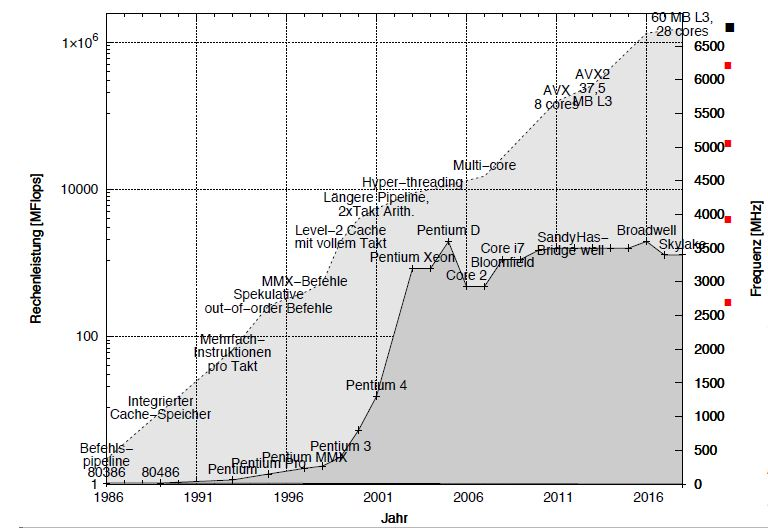
\includegraphics[width=7cm]{fig/moore.JPG}
	\caption{Mooresches Gesetz}
	\label{fig:moore}
\end{figure}
Auffallend in Abbildung \ref{fig:moore} ist, dass die Frequenz der einzelnen Kerne seit einigen Jahren nicht mehr zunimmt. Dies bedeutet, dass das Wachstum nicht mehr durch das Steigern von Leistung, sondern durch Caching und das Parallelisieren z.B. �ber mehrere CPU-Kerne bestimmt wird. Ein neuer Prozessor hat also nicht mehr Leistung als ein �lterer, sondern er besteht aus mehr CPU-Kernen. Gerade im Bereich des Hochleistungsrechnen ergibt sich daraus, dass viele Anwendungen parallel ausgef�hrt werden.

\section{Speicherzugriffe}
\label{sec:speicherzugriffe}

Mit Speicherzugriffen kann ein Prozessor Daten aus einem Speicher holen und auch in ihn schreiben. Dabei kann im Wesentlichen zwischen Registern, Caches, Hauptspeicher und Festplatte unterschieden werden. Wo der Zugriff auf Register ohne grosse Latenzen m�glich ist, ist der Zugriff auf andere Speicher deutlich langsamer. Die Zugriffszeiten sind in Tabelle \ref{tab:Speicher} vergleichend dargestellt. Faktor 10 bedeutet hierbei, dass die CPU zehn mal schneller auf ein Register als auf den L3-Cache zugreifen kann. 
\begin{table}[h]
	\centering
	\begin{tabular}{l|l}
		\textbf{Speicher} & \textbf{Zugriffszeit} \\
		\hline
		CPU zu L3-Cache & Faktor 10 \\
		\hline
		CPU zu Hauptspeicher & Faktor 100 bis 1000 \\
		\hline
		CPU zu Festplatte & Faktor 1000 bis 1000000 \\
	\end{tabular}
	\caption{Speicherzugriffe}
	\label{tab:Speicher}
\end{table}

Aufgrund dieser Geschwindigkeitsunterschiede ist es notwendig den Zugriff auf Speicher m�glichst effizient zu gestalten, da es sonst zu erheblichen Engp�ssen in Programmabl�ufen kommen kann.

\section{Dateisysteme}
\label{sec:dateisysteme}

Der Zugriff auf Dateien, welche auf der Festplatte liegen, geschieht �ber Dateisysteme. Mit einem Dateisystem wird dabei die Ablage dieser Dateien auf der Festplatte organisiert. Damit k�nnen diese dann gespeichert, gelesen, ver�ndert oder gel�scht werden.
Beim Zugriff auf Dateien kann im Wesentlichen zwischen seriellem und parallelem File-IO unterschieden werden. Die Unterscheidung hierbei liegt darin, wie parallel ausgef�hrte Programme auf Dateien zugreifen.

\subsection{Serieller IO}
\label{subsec:serieller_io}

Beim seriellen IO l�uft der komplette IO �ber einen Masterprozess. Dies bedeutet, dass Programme nicht gleichzeitig auf eine Datei zugreifen k�nnen. Dies ist in Abbildung \ref{fig:serial} ersichtlich.
\begin{figure}[h]
	\centering
	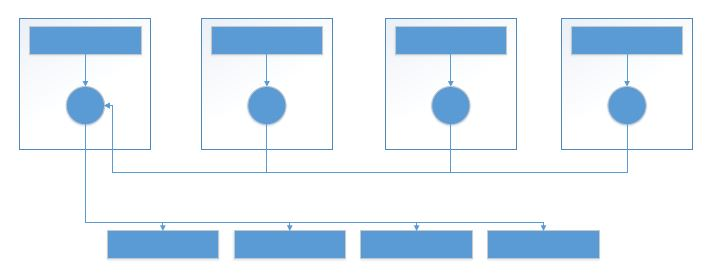
\includegraphics[width=7cm]{fig/SerialIO.JPG}
	\caption{Serial IO \cite{Cazes.26.09.2013}}
	\label{fig:serial}
\end{figure}

In Abbildung \ref{fig:serial} ist zu erkennen, dass es zu starken Engp�ssen kommen kann, wenn mehrere Programme gleichzeitig auf eine Datei zugreifen wollen. Diese Art des IO stellt daher auf kleinen Desktop-Computern mit nur wenigen parallelen Programmen kein Problem dar, im Bereich des High-Performance-Computing mit vielen parallelen Programmen sollte aber auf andere Methoden zur�ckgegriffen werden.\cite{Cazes.26.09.2013}

\subsection{Paralleler IO}
\label{subsec:paralleler_io}

Im Gegensatz zum seriellen IO ist es beim parallelen IO m�glich, dass mehrere Prozesse zeitgleich auf eine Datei zugreifen k�nnen. Dies ist in \ref{fig:parallel} dargestellt. Darin wird ersichtlich, dass der IO nicht mehr �ber einen Masterprozess l�uft, sondern, dass die einzelnen Prozesse ihren IO unabh�ngig voneinander durchf�hren.
\begin{figure}[h]
	\centering
	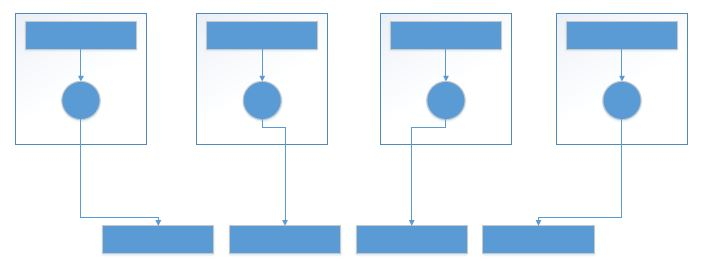
\includegraphics[width=7cm]{fig/ParallelIO.JPG}
	\caption{Parallel IO \cite{Cazes.26.09.2013}}
	\label{fig:parallel}
\end{figure}
Der Vorteil hierbei liegt darin, dass die einzelnen Prozesse parallel auf Dateien zugreifen bzw. in diese schreiben k�nnen. Gerade im Bereich des High-Performance-Computing mit sehr vielen parallelen Prozessen stellt dies einen wichtigen Vorteil dar.\cite{Cazes.26.09.2013}

\subsection{POSIX IO}
\label{subsec:posix_io}

POSIX-IO ist der IO-Part des POSIX-Standards. Der POSIX-Standard ist ein Standard f�r die Kommunikation von Prozessen mit dem Betriebssystem. POSIX-IO beschreibt dabei verschiedene Funktionen, �ber welche Programme in einem POSIX-Betriebssystem auf Dateien zugreifen k�nnen. Mit diesen Funktionen kann ein Programm dann bspw. eine Datei �ffnen, in diese schreiben und diese anschliessend wieder schliessen. Der Zugriff auf POSIX-IO-Funktionen geschieht zumeist �ber die glibc. Die glibc ist eine Bibliothek, welche Systemaufrufe als C-Funktionen bereitstellt. �ber diese C-Funktionen k�nnen Programme dann Systemaufrufe durchf�hren.

POSIX-IO eignet sich gut f�r den Einsatz im Bereich von Desktop-PCs mit nur vergleichsweise wenigen parallelen Prozessen. F�r den Einsatz im HPC-Bereich hat POSIX-IO jedoch einige Schwachstellen, welche im Folgenden erl�utert werden sollen.

\subsubsection{Metadaten}
\label{subsubsec:metadaten}

Dateien auf einem POSIX-Dateisystem m�ssen eine Vielzahl an Metadaten besitzen. Sollen Informationen �ber eine Datei angezeigt werden, m�ssen diese Metadaten ausgelesen werden. Auf HPC-Systemen kann dies einen Nachteil darstellen, da das Auslesen der Metadaten von vielen Dateien mitunter sehr lange dauert\cite{Layton.02.03.2010}.

Ein weiterer Nachteil der Metadaten liegt darin, dass diese bei jedem Schreibvorgang aktualisiert werden m�ssen. Dies kostet sehr viel Zeit, wodurch Schreibvorg�nge in Bezug auf die Geschwindigkeit erheblich eingeschr�nkt werden.

Dar�ber hinaus sind die Metadaten in POSIX-IO sehr unflexibel, da s�mtliche Dateien alle Metadaten besitzen m�ssen und nicht bspw. Metadaten f�r alle Dateien in einem Ordner gelten k�nnen.

\subsubsection{File-Descriptoren}
\label{subsubsec:file-descriptoren}

Bevor eine Datei in POSIX gelesen werden kann, muss diese zun�chst ge�ffnet werden, um einen File-Descriptor zu erhalten. In diesem File-Descriptor wird der Status der Datei gespeichert. Wird eine Datei wieder geschlossen, wird der File-Descriptor wieder freigegeben.

Der Nachteil von File-Descriptoren kommt zum Tragen, wenn viele Prozesse gleichzeitig auf ein Dateisystem zugreifen wollen. Dann muss das Betriebssystem sehr viele File-Descriptoren parallel verwalten, wodurch bspw. das �ffnen einer Datei immer langsamer wird, je mehr Prozesse parallel auf das Dateisystem zugreifen. In Abbildung \ref{fig:posix} ist dabei ersichtlich, dass das �ffnen einer Datei linear langsamer wird, je mehr parallele Prozesse auf das Dateisystem zugreifen.
\begin{figure}[h]
	\centering
	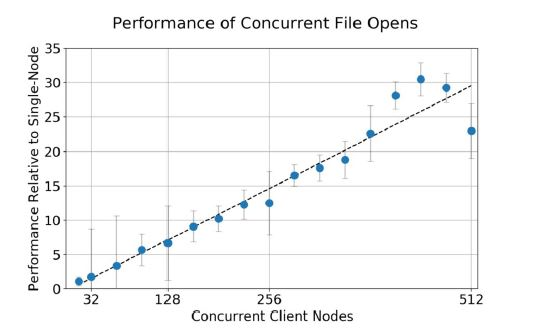
\includegraphics[width=7cm]{fig/PosixIO.JPG}
	\caption{\"Offnen einer Datei bei POSIX-IO \cite{Lockwood.11.09.2017}}
	\label{fig:posix}
\end{figure}

\subsubsection{Konsistenz}
\label{subsubsec:konsistenz}

Das Schreiben in eine Datei muss in POSIX konsistent sein. Dies bedeutet, dass das Schreiben die Ausf�hrung einer Applikation so lange blockiert, bis sichergestellt ist, dass ein Lesezugriff das neu geschriebene sieht. Dies hat wiederum den Nachteil zur Folge, dass im Ausf�hren von Applikationen durch das Schreiben in eine Datei starke Latenzzeiten entstehen. Im HPC-Bereich mit vielen parallelen Applikationen stellt dies ein grosses Problem dar, wenn viele Prozesse gleichzeitig in Dateien schreiben wollen.
\cite{Lockwood.11.09.2017}

\subsection{MPI-IO}
\label{subsec:mpi-io}

MPI-IO ist der IO-Part des Message Passing Interface (MPI). MPI-IO ist dabei eine sog. Middleware, welche i.d.R. nicht direkt von Anwendungen sondern nur indirekt durch h�here Schichten genutzt wird. Es definiert somit einen Standard f�r parallele IO-Operationen in einer MPI-Applikation. Im Gegensatz zu POSIX-IO ist der Zugriff auf Dateien hierbei nicht Bytestrom- sondern elementorientiert. Der Aufbau einer Datei in MPI-IO ist in Abbildung \ref{fig:dateityp} und in Abbildung \ref{fig:dateisicht} ersichtlich. Eine Datei wird dabei in sog. Fliessen aufgeteilt. Auf diese Fliessen kann �ber einen Dateityp zugegriffen werden. Ein Dateityp beschreibt ein Muster an Fliessen, welches sich �ber Teile der Datei oder �ber die ganze Datei wiederholt. Ein solches Muster ist in Abbildung \ref{fig:dateityp} dargestellt. Jede Fliesse im Muster besteht wiederum aus einem elementaren Typ. Der elementare Typ ist der Datentyp �ber welchen auf die Datei zugegriffen werden kann. Ein Prozess, der auf die Datei �ber diesen Dateityp zugreift kann somit auf alle Fliessen zugreifen, welche in diesem Muster liegen.


\begin{figure}[h]
	\centering
	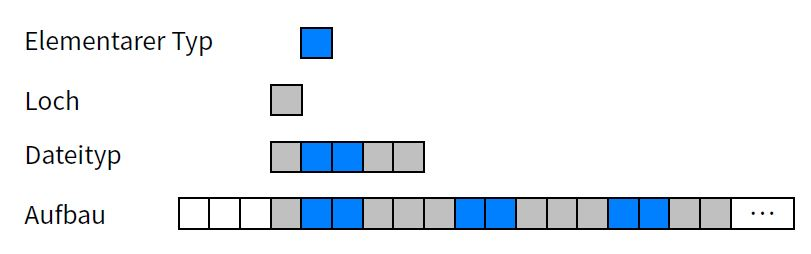
\includegraphics[width=7cm]{fig/Dateityp.JPG}
	\caption{Dateityp bei MPI-IO \cite{Kuhn.13.05.2016}}
	\label{fig:dateityp}
\end{figure}

In Abbildung \ref{fig:dateisicht} ist der Aufbau einer Datei aus Sicht von Prozessen dargestellt. Dies wird auch als Dateisicht bezeichnet. Jeder Prozess greift damit �ber einen anderen Dateityp auf die Datei zu, wodurch mehrere Prozesse gleichzeitig auf die Datei zugreifen k�nnen. Dass mehrere Prozesse zeitgleich auf Teile einer Datei zugreifen, ist in dieser Form in POSIX-IO nicht m�glich und stellt damit einen entscheidenden Vorteil von MPI-IO gegen�ber POSIX-IO dar.

\begin{figure}[h]
	\centering
	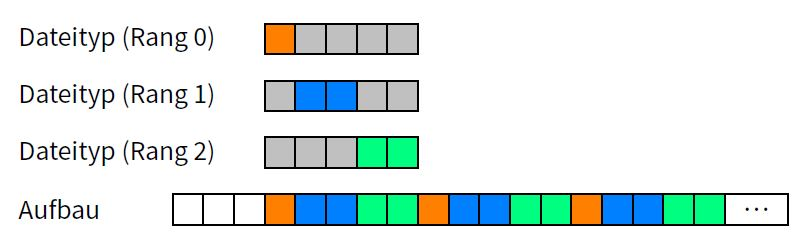
\includegraphics[width=7cm]{fig/Dateisicht.JPG}
	\caption{Dateisicht bei MPI-IO \cite{Kuhn.13.05.2016}}
	\label{fig:dateisicht}
\end{figure}

MPI-IO stellt im High-Performance-Bereich eine gute Alternative zu POSIX dar, da damit mehrere Prozesse zeitgleich auf eine Datei zugreifen bzw. in diese schreiben k�nnen. Die popul�rste Implementierung von MPI-IO ist ROMIO. MPI-IO bildet dar�ber hinaus die Basis vieler IO-Systeme wie bspw. HDF.\cite{Corbett.1995}\cite{Kuhn.13.05.2016}
% Bsp. eines Hauptteils

\chapter{Einf�hrung}
\label{sec:grundl}

\chapter{Stand der Technik}
\label{sec:tech}

\chapter{Architektur}
\label{sec:real}

\chapter{Umsetzung}
\label{sec:umsetz}

\chapter{Aktueller Stand}
\label{sec:ergeb}


\chapter{Zusammenfassung und Ausblick}
\label{sec:schluss}

Nach einer kurzen Evaluation von verf�gbaren Werkzeugen zur Analyse von File-IO wurden diese als unzureichend f�r den angestrebten Zweck beurteilt. Lediglich Darshan erf�llt die grundlegenden Anforderungen. Mit Darshan k�nnen POSIX-IO und MPI-IO in eine Log-Datei protokolliert werden. Diese Datei kann dann durch ein Analyseprogramm augewertet werden. Darshan unterst�tzt jedoch nur POSIX-IO und MPI-IO. Andere Arten von Dateizugriffen werden nicht ber�cksichtigt. Diese sind allerdings im HPC-Bereich von entscheidender Bedeutung. So erfordert eine hochparallelisierte Kommunikation zu Dateien zum Beispiel ein Dateisystem wie Lustre. Dieses bringt entsprechend eigene File-IO-Funktionen mit sich, welche �ber Darshan nicht protokolliert werden k�nnen. Zudem schreibt Darshan die Protokolldateien in einem Bin�rformat. Dieses ist entsprechend seiner Natur nicht leicht aus anderen Anwendungen heraus zu nutzen. Insbesondere bei der Verwendung von Programmiersprachen welche die bin�re Kodierung vor dem Entwickler verbergen (wie zum Beispiel Java) stellt das Bin�rformat ein unerw�nschtes Hindernis dar.

Nach der Evaluation wurde daher mit dem Entwurf einer eigenen L�sung begonnen. Dabei lag der Fokus im ersten Schritt auf den Wrappern. Deren Architektur und das Datenformat der Protokollierung wurden nach Gesichtspunkten der Performance und der Nutz- und Erweiterbarkeit gew�hlt. Dabei ergaben sich f�r das Abfangen der File-IO-Funktionsaufrufe �hnliche Ans�tze wie in Darshan, w�hrend die Protokollierung andere Ans�tze verfolgt. Neben der Architektur der Wrapper wurde f�r das gesamte System eine erste grobe Architektur festgelegt.

Welche Daten durch die ersten Wrapper f�r einfache Analysen gebraucht werden, wurde durch eine Betrachtung m�glicher File-IO-Konstellatione ermittelt. Abh�ngig von den k�nftig im Projekt geplanten Analysen m�ssen jedoch weitere Daten protokolliert werden. Diese Erkenntnis wurde beim Entwurf der Wrapper und insbesondere bei der Wahl des Datenformats ber�cksichtigt.

Als Datenformat f�r die Protokollierung wurde JSON gew�hlt. Dieses Format erm�glicht eine Enfache Nutzung der protokollierten Daten mittels unterschiedlicher Programmiersprachen aus verschiedenen Plattformen heraus. Dabei h�lt sich der Overhead beim Protokollieren im Vergleich zu anderen Formaten in Grenze. JSON bietet zudem die M�glichkeit die Protokollierung einfach zu erweitern. Werden nachtr�glich durch Wrapper zus�tzliche Daten ben�tigt, so k�nnen diese im JSON-Format hinzugef�gt werden, ohne dass dies ein Auslesen der Datei beeintr�chtigt.

Nach einem erfolgreichen Test des Konzepts der Wrapper wurde mittlerweile mit der Implementierung begonnen. Dabei liegt der Fokus zun�chst auf POSIX-IO und MPI-IO. Im kommenden Semester ist geplant die Wrapper weitgehend fertig zu stellen. Nach erfolgreicher Implementierung der Wrapper wird mit der Umsetzung der restlichen Komponenten begonnen.

Da bei dem Entwurf einer eigenen L�sung f�r die Wrapper zum Protokollieren des File-IOs �hnliche Ans�tze wie in Darshan gew�hlt wurden, ist eine weitergehende Analyse von Darshan bez�glich der Performance sinnvoll. Hier wird insbesondere ein Vergleich zwischen der im Rahmen dieses Projektes erstellten libiotrace und Darhans libdarshan.so angestrebt. Mit dieser Aufgabe kann begonnen werden, sobald die Wrapper einen mit Darshan vergleichbaren Funktionsumfang erreicht haben.

% % %%%%%% Anhang
\appendix
\chapter{Anhang}
\label{sec:a-kapitel}

\lstset{literate=
  {á}{{\'a}}1 {é}{{\'e}}1 {í}{{\'i}}1 {ó}{{\'o}}1 {ú}{{\'u}}1
  {Á}{{\'A}}1 {É}{{\'E}}1 {Í}{{\'I}}1 {Ó}{{\'O}}1 {Ú}{{\'U}}1
  {� }{{\`a}}1 {è}{{\`e}}1 {ì}{{\`i}}1 {ò}{{\`o}}1 {ù}{{\`u}}1
  {À}{{\`A}}1 {È}{{\'E}}1 {Ì}{{\`I}}1 {Ò}{{\`O}}1 {Ù}{{\`U}}1
  {ä}{{\"a}}1 {ë}{{\"e}}1 {ï}{{\"i}}1 {ö}{{\"o}}1 {ü}{{\"u}}1
  {Ä}{{\"A}}1 {Ë}{{\"E}}1 {Ï}{{\"I}}1 {Ö}{{\"O}}1 {Ü}{{\"U}}1
  {â}{{\^a}}1 {ê}{{\^e}}1 {î}{{\^i}}1 {ô}{{\^o}}1 {û}{{\^u}}1
  {Â}{{\^A}}1 {Ê}{{\^E}}1 {Î}{{\^I}}1 {Ô}{{\^O}}1 {Û}{{\^U}}1
  {œ}{{\oe}}1 {Œ}{{\OE}}1 {æ}{{\ae}}1 {Æ}{{\AE}}1 {ß}{{\ss}}1
  {ű}{{\H{u}}}1 {Ű}{{\H{U}}}1 {ő}{{\H{o}}}1 {Ő}{{\H{O}}}1
  {ç}{{\c c}}1 {Ç}{{\c C}}1 {ø}{{\o}}1 {å}{{\r a}}1 {Å}{{\r A}}1
  {€}{{\euro}}1 {£}{{\pounds}}1 {«}{{\guillemotleft}}1
  {»}{{\guillemotright}}1 {ñ}{{\~n}}1 {Ñ}{{\~N}}1 {¿}{{?`}}1,
  basicstyle=\fontsize{10}{12}\selectfont,
  breaklines=true,
  backgroundcolor=\color{white},
  keywordstyle=\color{blue},
  stringstyle=\color{orange},
  commentstyle=\color{teal},
  morecomment=[l][\color{magenta}]{\#},
  %identifierstyle=\color{olive}
}
\lstloadlanguages{bash,C++,C}

\section{Testprogramm OpenMP}
\label{sec:testprogramm_openmp}

\lstinputlisting[language=C,numbers=left,numberstyle=\tiny]{source/test.c}

\section{dynamischer Wrapper mit zentraler Buffer}
\label{sec:dynamischer_wrapper_mit_zentraler_buffer}

\lstinputlisting[language=C,numbers=left,numberstyle=\tiny]{source/wrap-preload_example.c}

\section{statischer Wrapper}
\label{sec:statischer_wrapper}

Die Funktino writeData ist im folgenden Beispiel nicht definiert. Sie kann analog zu einem dynamischen Wrapper implementiert werden \verw{sec:dynamischer_wrapper_mit_zentraler_buffer}.
\lstinputlisting[language=C,numbers=left,numberstyle=\tiny]{source/wrap-link_example.c}

\section{linken statischer Wrapper}
\label{sec:linken_statischer_wrapper}

Im folgenden Beispiel wurde wrap-link.o aus einem statischen Wrapper \verw{sec:statischer_wrapper} und test-link.o aus einem Testprogramm \verw{sec:testprogramm_openmp} kompiliert.
\lstinputlisting[language=C,numbers=left,numberstyle=\tiny]{source/wrap-link_link.txt}

% % %%%%%% Literaturverzeichnis (darf im deutschen nicht in den Anhang!)
% Einfaches Literaturverzeichnis

\bibliography{bib/bib}{}
\bibliographystyle{plain}
% Literaturverzeichnis mit Bibtex
%\bibliography{bib/bib}

% %  Inhalt ENDE %%%%%%%%%%%%%%%%%%%%%%%%%%%%%%%%%%%%%%%%%%%%%%%%%%%%%%%%%%
\end{document}
